%% This is file `DEMO-TUDaThesis.tex' version 2.09 (2020/03/13),
%% it is part of
%% TUDa-CI -- Corporate Design for TU Darmstadt
%%  --  --  --  --  --  --  --  --  --  --  --  --  --  --  --  --  --  --  --  --  --  --  --  --  -- -
%%
%%  Copyright (C) 2018--2020 by Marei Peischl <marei@peitex.de>
%%
%% ============================================================================
%% This work may be distributed and/or modified under the
%% conditions of the LaTeX Project Public License, either version 1.3c
%% of this license or (at your option) any later version.
%% The latest version of this license is in
%% http://www.latex-project.org/lppl.txt
%% and version 1.3c or later is part of all distributions of LaTeX
%% version 2008/05/04 or later.
%%
%% This work has the LPPL maintenance status `maintained'.
%%
%% The Current Maintainers of this work are
%%   Marei Peischl <tuda-ci@peitex.de>
%%   Markus Lazanowski <latex@ce.tu-darmstadt.de>
%%
%% The development respository can be found at
%% https://github.com/tudace/tuda_latex_templates
%% Please use the issue tracker for feedback!
%%
%% ============================================================================
%%
% !TeX program = lualatex
%%

\documentclass[
	english,
	ruledheaders=section,%Ebene bis zu der die Überschriften mit Linien abgetrennt werden, vgl. DEMO-TUDaPub
	class=report,% Basisdokumentenklasse. Wählt die Korrespondierende KOMA-Script Klasse
	thesis={type=bachelor},% Dokumententyp Thesis, für Dissertationen siehe die Demo-Datei DEMO-TUDaPhd
	accentcolor=1b,% Auswahl der Akzentfarbe
	custommargins=true,% Ränder werden mithilfe von typearea automatisch berechnet
	marginpar=false,% Kopfzeile und Fußzeile erstrecken sich nicht über die Randnotizspalte
	%BCOR=1mm,%Bindekorrektur, falls notwendig
	parskip=half-,%Absatzkennzeichnung durch Abstand vgl. KOMA-Sript
	fontsize=11pt,%Basisschriftgröße laut Corporate Design ist mit 9pt häufig zu klein
	DIV=14,
%	logofile=example-image, %Falls die Logo Dateien nicht vorliegen
]{tudapub}
\usepackage{datetime2}


% Der folgende Block ist nur bei pdfTeX auf Versionen vor April 2018 notwendig
%\usepackage{iftex}
%\ifPDFTeX
%	\usepackage[utf8]{inputenc}%kompatibilität mit TeX Versionen vor April 2018
%\fi

%%%%%%%%%%%%%%%%%%%
%Sprachanpassung & Verbesserte Trennregeln
%%%%%%%%%%%%%%%%%%%
\usepackage[ngerman, main=english]{babel}
\usepackage[autostyle]{csquotes}% Anführungszeichen vereinfacht
\usepackage{microtype}
\usepackage[super]{nth} % converts Dec \nth{1} to Dec 1st (with st as superscript)

%%%%%%%%%%%%%%%%%%%
%Literaturverzeichnis
%%%%%%%%%%%%%%%%%%%
\usepackage[style=apa,backend=biber]{biblatex}    % Literaturverzeichnis
\bibliography{references}
\AtBeginBibliography{\setcounter{maxnames}{10}} % Im Literaturverzeichnis nenne mehr als 2 Autoren
\counterwithout{footnote}{chapter} % Zähle Fußnoten über gesamtes Dokument hoch


%%%%%%%%%%%%%%%%%%%
%Paketvorschläge Tabellen
%%%%%%%%%%%%%%%%%%%
%\usepackage{array}     % Basispaket für Tabellenkonfiguration, wird von den folgenden automatisch geladen
\usepackage{tabularx}   % Tabellen, die sich automatisch der Breite anpassen
\usepackage{longtable} % Mehrseitige Tabellen
\usepackage{xtab,afterpage}
%\usepackage{xltabular} % Mehrseitige Tabellen mit anpassarer Breite
\usepackage{booktabs}   % Verbesserte Möglichkeiten für Tabellenlayout über horizontale Linien
\usepackage{tikz}       % Graphen zeichnen
\usepackage{enumitem, hyperref}   % for referencing in enumerate und description
\usepackage{amsmath}    % https://tex.stackexchange.com/questions/32140/how-to-write-a-function-piecewise-with-bracket-outside
% https://texblog.org/2012/03/21/cross-referencing-list-items/
\usepackage[acronym,shortcuts,nonumberlist,nomain]{glossaries} % for Abbreviations (Acronyms)

%%%%%%%%%%%%%%%%%%%
%Paketvorschläge Mathematik
%%%%%%%%%%%%%%%%%%%
%\usepackage{mathtools} % erweiterte Fassung von amsmath
%\usepackage{amssymb}   % erweiterter Zeichensatz
%\usepackage{siunitx}   % Einheiten

% Customs
%\usepackage[singlespacing]{setspace}
\usepackage[]{setspace}
%\usepackage[printonlyused]{acronym}

%Formatierungen für Beispiele in diesem Dokument. Im Allgemeinen nicht notwendig!
\let\file\texttt
\let\code\texttt
\let\tbs\textbackslash

\usepackage{pifont}% Zapf-Dingbats Symbole
\newcommand*{\FeatureTrue}{\ding{52}}
\newcommand*{\FeatureFalse}{\ding{56}}

\makeglossaries

\begin{document}

\Metadata{
	title=Automatic evaluation of Enterprise-GenAI Applications success,
	author=Marcel Pfeiffer
}

\pagenumbering{gobble}

\title{Automatic evaluation of Enterprise-GenAI Applications success}

\studentID{2912332}
\author[M. Pfeiffer]{Marcel Pfeiffer}%optionales Argument ist die Signatur,
\birthplace{Koblenz}%Geburtsort, bei Dissertationen zwingend notwendig
\reviewer{Prof. Dr. Peter Buxmann \and Prof. Dr. X Y}%Gutachter

%Diese Felder erden untereinander auf der Titelseite platziert.
%\department ist eine notwendige Angabe, siehe auch dem Abschnitt `Abweichung von den Vorgaben für die Titelseite'
\department{wi} % Das Kürzel wird automatisch ersetzt und als Studienfach gewählt, siehe Liste der Kürzel im Dokument.
\institute{Wirtschatsinformatik}
\group{Software \& Digital Business}

\submissiondate{\today}
\examdate{\today}

%	\tuprints{urn=1234,printid=12345}
%	\dedication{Für alle, die \TeX{} nutzen.}

\maketitle

\affidavit


% --  --  --  --  --  --  --  --  --  --  --  --  --  --  --  --  --  --  --  --  --  --  -- %
% --  --  --  --  --  --  --  --  -- -- Abstract  --  --  --  --  --  --  --  --  --  -- %
% --  --  --  --  --  --  --  --  --  --  --  --  --  --  --  --  --  --  --  --  --  --  -- %
\chapter*{Abstract}
Generative AI (GenAI) and especially Retrieval Augmented Generation (RAG) applications revolutionize the modern business world. Yet the success of RAG applications in enterprises is not guaranteed and the systems need to be maintained to generate high quality outputs. Without systematic evaluation, system administrators lack the data-driven insights necessary to identify weaknesses and develop improvements. This bachelor's thesis addresses this challenge through the design, development, and evaluation of an analytics dashboard for the automatic success measurement of an enterprise GenAI application.

Following the IS Success Model (ISSM) by DeLone and McLean an Information System's success is determined by three quality factors: \textit{the information quality, the system quality and the service quality}. However, the current evaluation frameworks for RAG systems like RAGAS or ARES focus only on the \textit{information quality} provided by the system. Based on the ISSM an integrated dashboard was created in close collaboration with a development team applying the Design Science Research methodology. It offers administrators insights into all three quality dimensions to provide a more holistic perspective on RAG success. The core features implemented include the AI-based evaluation of answer and document quality, the visualization of topics appearing in the user requests and the analysis of the most important task types. Combined views allow for the direct correlation of quality metrics with specific topics and tasks to identify problems and optimization potential.

An evaluation with the development team confirmed the dashboard's significant value and practical relevance. Furthermore, a cost analysis revealed that the analytics functionalities add an increase of approximately 20\% to the already existing LLM-related costs. This cost increase is justified by the benefit provided by the dashboard. Despite the positive feedback by the development, the implemented dashboard should undergo practical testing with end users to enhance its capabilities. In summary, this work provides an internally validated foundation for the data-driven success measurement of enterprise GenAI systems and establishes the concept of a holistic perspective on RAG success.

\tableofcontents


\pagenumbering{Roman}

% --  --  --  --  --  --  --  --  --  --  --  --  --  --  --  --  --  --  --  --  --  --  -- %
% --  --  --  --  --  --  --  -- -- List of Figures  --  --  --  --  --  --  --  -- --%
% --  --  --  --  --  --  --  --  --  --  --  --  --  --  --  --  --  --  --  --  --  --  -- %

\listoffigures
\addcontentsline{toc}{chapter}{Abbildungsverzeichnis}           %Kapitel bekommt keine Nummerierung und wird trotzdem
                                                                %ins Inhaltsverzeichnis aufgenommen
% --  --  --  --  --  --  --  --  --  --  --  --  --  --  --  --  --  --  --  --  --  --  -- %
% --  --  --  --  --  --  --  --  --  List of Tables  --  --  --  --  --  --  --  -- --%
% --  --  --  --  --  --  --  --  --  --  --  --  --  --  --  --  --  --  --  --  --  --  -- %

\listoftables
\addcontentsline{toc}{chapter}{Tabellenverzeichnis}           %Kapitel bekommt keine Nummerierung und wird trotzdem
                                                                %ins Inhaltsverzeichnis aufgenommen

% --  --  --  --  --  --  --  --  --  --  --  --  --  --  --  --  --  --  --  --  --  --  -- %
% --  --  --  --  --  --  --  -- -- List of Abbreviations  --  --  --  --  --  --  -- --%
% --  --  --  --  --  --  --  --  --  --  --  --  --  --  --  --  --  --  --  --  --  --  -- %
\chapter*{List of abbreviations}
\addcontentsline{toc}{chapter}{List of abbreviations}            %Kapitel bekommt keine Nummerierung und wird trotzdem
                                                                %ins Inhaltsverzeichnis aufgenommen

\begin{xtabular}{ll}
AI & Artificial Intelligence\\
ARES & Automatic RAG Evaluation and Scoring \\
DSR & Design Science Research\\
DSGVO & Datenschutz-Grundverordnung (General Data Protection Regulation)\\
GCP & Google Cloud Platform\\
GDPR & General Data Protection Regulation\\
GenAI & Generative AI\\
HDBSCAN & Hierarchical Density-Based Spatial Clustering of Applications with Noise\\
IS & Information Systems\\
ISSM & Information Systems Success Model\\
KM & Knowledge Management\\
KMS & Knowledge Management System\\
LLM & Large Language Model\\
ML & Machine Learning\\
PCA & Principal Component Analysis \\
PEU & Perceived Ease of Use\\
PU & Perceived Usefulness\\
RAG & Retrieval-Augmented Generation\\
RAGAS & Retrieval-Augmented Generation Assessment \\
TAM & Technology Acceptance Model\\
t-SNE & t-distributed Stochastic Neighbor Embedding \\
UMAP & Uniform Manifold Approximation and Projection\\
\end{xtabular} 

% --  --  --  --  --  --  --  --  --  --  --  --  --  --  --  --  --  --  --  --  --  --  -- %
% --  --  --  --  --  --  --  --  -- - Introduction  --  --  --  --  --  --  --  --  -- %
% --  --  --  --  --  --  --  --  --  --  --  --  --  --  --  --  --  --  --  --  --  --  -- %

\onehalfspacing
% Umstellen auf arabische Seitenzahlen. Die Anzahl der bisherigen
% Seiten wird zwischengespeichert, da die römische Nummerierung am
% Ende des Dokuments fortgesetzt werden soll.
\newcounter{seitenzahlroemisch}
\setcounter{seitenzahlroemisch}{\value{page}}
\pagenumbering{arabic}

\chapter{Introduction}
ChatGPT reached 1 million users within 5 days after its launch in 2022 which was only exceeded by Threads in 2023 \parencite{Brandt2023}. Today ChatGPT provides benefits for 800 million weekly users \parencite{Huber2025} and thus has become an established Generative AI (GenAI) tool. GenAI bares high potential not only for the private sector but also for the modern business world. Projections underscore this, suggesting that GenAI could increase Germany's GDP by up to \EUR{585} billion by 2040 \parencite[p.~12]{McKinsey2023}. Furthermore for enterprise applications, \textbf{Retrieval-Augmented Generation (RAG)} has emerged as a particularly suitable technology by connecting large language models (LLMs) to company-specific proprietary knowledge bases \parencite[p.~6]{Sahin2024LLM_proceedings}. Connecting and bounding LLMs to proprietary knowledge bases not only enables them to access up-to-date company data but also enhances transparency and reduces the likelihood of hallucinations, as the company data serves as the ground truth \parencite{GoogleCloudRAG}.

However, the success of enterprise RAG applications typically requires some effort, including the use of specialized RAG pipelines or connecting various APIs to the RAG system, to implement them effectively \parencite[p.~6--7]{Bruckhaus2024RAG}. Common failure points include the system failing to provide an answer even though the information is available, generating a false answer by misinterpreting context or returning an incomplete response \parencite[p.~4]{Barnett_Kurniawan_Thudumu_Brannelly_Abdelrazek_2024}. As organizations invest in and deploy these powerful but complex systems, a critical management challenge arises: How can the success of a GenAI application be measured and monitored over time? Without systematic evaluation, system administrators lack the data-driven insights needed to identify weaknesses, justify improvements, and ensure that the system delivers a positive return on investment.

This thesis addresses this management challenge directly. It documents the design, development, and evaluation of an analytics dashboard designed to measure the success of an enterprise GenAI application automatically. Following the Information Systems Success Model \parencite{DeloneMcLean2003ISSuccessTenYearUpdate}, success can be measured using three quality metrics: \textit{information quality}, \textit{system quality}, and \textit{service quality}. However, most RAG evaluation frameworks like RAGAS \parencite{Es_James_Espinosa_Anke_Schockaert_2024} or ARES \parencite{Saad_Falcon_Khattab_Potts_Zaharia_2024} only include the information quality provided by the system. To move beyond this narrow perspective on IS success, this study employs a Design Science Research methodology following \cite{Peffers2007} to conceptualize and implement a dashboard based on a more holistic perspective.
% --  --  --  --  --  --  --  --  --  --  --  --  --  --  --  --  --  --  --  --  --  --  -- %
% --  --  --  --  --  --  --  --  --  --  Theoretical Background  --  --  --  --  -- %
% --  --  --  --  --  --  --  --  --  --  --  --  --  --  --  --  --  --  --  --  --  --  -- %
\chapter{Theoretical Background}
In order to gain a deeper understanding of what determines the success of an enterprise Gen-AI system, we will first look at the success of IS in general. Afterwards, we will dive deeper into the context of KMS - specifically enterprise GenAI systems and apply the more general theories to them. This will help us define and categorize the software features we are going to implement during our artifact development.
\section{Technology acceptance and IS success}
To better understand the success of IS we will have a look at two models. The technology acceptance model (TAM) \parencite{Davis1989} deals with the question, which determinants lead to the acceptance and use of an IS by a single user, whereas the IS success model \parencite{DeloneMcLean2003ISSuccessTenYearUpdate} focuses on the success of an IS in an organizational context.
\begin{figure}[h!]
    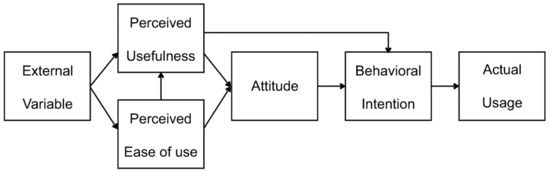
\includegraphics[width=1\linewidth]{images/TAM.png}
    \caption{Technology acceptance model}
    \label{fig:enter-label}
\end{figure}
\\
Looking at the TAM two determinants influence the use of an IS - the \textit{perceived usefulness} (PU) and the \textit{perceived ease of use} (PEU) \parencite{Davis1989}. Both are influenced by external variables \parencite{Davis1989}. The PU describes the degree to which a person believes that using a particular system would be beneficial to them \parencite{Davis1989}. In an enterprise context this usually means the conviction that the use of the IS has a beneficial influence on the own job performance. The second determinant, the \textit{perceived ease of use} (PEU), refers to "the degree to which a person believes that using a particular system would be free of effort" \parencite[p.~320]{Davis1989}. This idea relates to the user's estimation of the mental effort required to learn and operate the system. If a system is intuitive, straightforward and does not require extensive training to use, it will be perceived as easy to use.\\ A crucial aspect of the TAM is the relationship between these two determinants. Davis argues that the PEU has a direct, positive influence on the PU. A system that is easier to use is also perceived as more useful, partly because the user can invest less effort in the mechanics of using the system and more in the actual task at hand. Both PU and PEU then influence the user's \textit{attitude toward using} the system, which in turn shapes the \textit{behavioral intention to use} and ultimately leads to the \textit{actual system use}. However, it is important to note that a consistent finding in TAM research is that PU has a significantly stronger influence on usage intention and actual use than PEU \parencite{Davis1989}. While ease of use is important, the ultimate driver for acceptance is the user's belief that the system will help them perform their job better.\\
\\
Now that we know which factors lead to the use of an IS by a single person, we will shift our perspective to the factors that determine its use and overall success within an organizational context.
Following DeLone and McLean \parencite{DeloneMcLean2003ISSuccessTenYearUpdate} there are 6 interrelated factors that determine the success of an IS in an organizational context: \textit{system quality, information quality, service quality, intention to use and actual system use, user satisfaction and the net benefits} of the IS.\\
\begin{figure}[h!]
    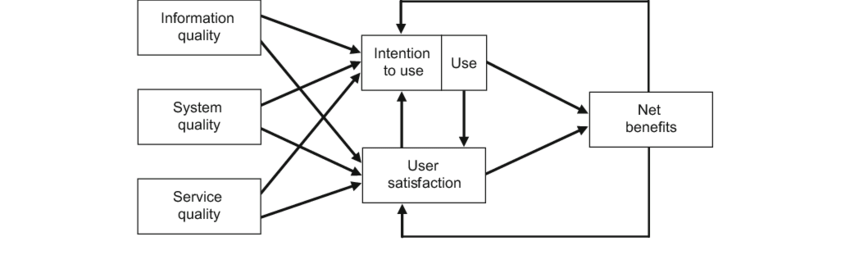
\includegraphics[width=1\linewidth]{images/ISSuccess.png}
    \caption{IS Success Model}
    \label{fig:enter-label}
\end{figure}
\\
\textit{System quality} means the quality of the IS in terms of technical performance. Typical measures for system quality would be, for example, response time, reliability, ease of use, or hardware utilization.\\
\textit{Information quality} refers to the quality of the information provided by the IS. This includes, for example, the usefulness, timeliness, precision, completeness, and relevance of the information provided by the system.\\
\textit{Service quality} means the quality of the support that users receive from the IS department or service provider. It became an important success dimension with the rise of end-user computing, where IS providers needed to provide services in addition to making them usable. This dimension is often measured by the support staff's responsiveness, assurance, and empathy.
\\
These three aspects of the quality of an information system directly influence the \textit{intention to use} and the actual \textit{system use} as well as the \textit{user satisfaction}. Here, it is important to differentiate between the two concepts of use. \textit{Intention to use} is an attitudinal measure, representing a user's plan to engage with a system. In contrast, \textit{system use} is a behavioral measure of the actual interaction, captured by metrics like frequency, duration, or the breadth of features used. This distinction is particularly crucial in an enterprise context. For a system where use is voluntary, a user's intention is a strong predictor of their actual use. However, if a system's use is mandatory, simply measuring that it is being used is not very meaningful, because the system has to be used anyway. In that scenario, assessing the nature of the use (e.g., are users leveraging advanced features?) or their underlying intention to use the system properly becomes a more telling indicator of true acceptance and success
\parencite{DeloneMcLean2003ISSuccessTenYearUpdate}. Both use and intention are linked with \textit{user satisfaction}. A positive experience during system use leads to higher satisfaction, which in turn reinforces the intention for continued and more extensive use in the future. In an organizational context, this user satisfaction is heavily influenced by the system's perceived impact on job performance, such as an increase in productivity. Therefore, the combination of active system use and high user satisfaction is what generates \textit{net benefits}.\\
This process, however, is not a one-way street. The model includes a crucial feedback loop: the \textit{net benefits} that users perceive will in turn influence their future \textit{user satisfaction} and \textit{intention to use}. When users see that a system is delivering real value, it reinforces their positive attitude towards the system. This creates a virtuous cycle, where a successful system's value is constantly reinforced and grows over time.\\

The Technology Acceptance Model (TAM) and the Information Systems Success Model (ISSM) address the same fundamental questions but from two different perspectives. The TAM focuses on the individual user, suggesting that a person will use a system more often if it provides value (\textit{perceived usefulness}) and is easy to operate (\textit{perceived ease of use}).
The ISSM, on the other hand, argues from a company's perspective. It concludes that three quality dimensions influence system success: \textit{information quality}, \textit{system quality}, and \textit{service quality}. These dimensions impact both \textit{user satisfaction} and \textit{ intention to use}, which drives \textit{actual system use}. Overall, the two models appear to be quite parallel to each other as both implement factors like how simple a system is to use and how beneficial the use is.

For this thesis, the ISSM provides a more practical framework. It offers specific, measurable dimensions rather than the TAM's general concept of \textit{external variables} and argues from a company's perspective. Therefore, we will use the ISSM to develop and categorize the quality measurements for the RAG application.

\newpage
\section{Knowledge Management System's success}
Now that we have a solid understanding of IS acceptance and success in general we are going to have a closer look at knowledge management systems (KMS). We'll start of with some definitions that will help us understand what knowledge, knowledge management (KM) and knowledge management systems (KMS) are. "Knowledge is a fluid mix of framed experience, values, contextual information, and expert insight that provides a framework for
evaluating and incorporating new experiences and information" \parencite[p.~15]{Davenport}. This means that knowledge is a key factor in decision-making processes, e.g., in enterprises. KM on the other hand "[...] is the practice of selectively applying knowledge from previous experiences of decision making to current and future decision making activities with the express purpose of improving the organization’s effectiveness" \parencite{Jennex2006WhatIsKM}. KMS in the end can be defined as "IT-based systems developed to support and enhance the organizational processes of knowledge creation, storage/retrieval, transfer and application". Overall, we can conclude that KMS are systems that support the decision-making process e.g. in a company by managing and selectively providing knowledge to their users. Since KMS are by definition a specialized form of IS we can simply apply the ISSM to them.\\
Following Jennex and Olfman we can extend the three quality factors to gain a better understanding
of knowledge management success \parencite{Jennex2006}.\\
\begin{figure}
    \centering
    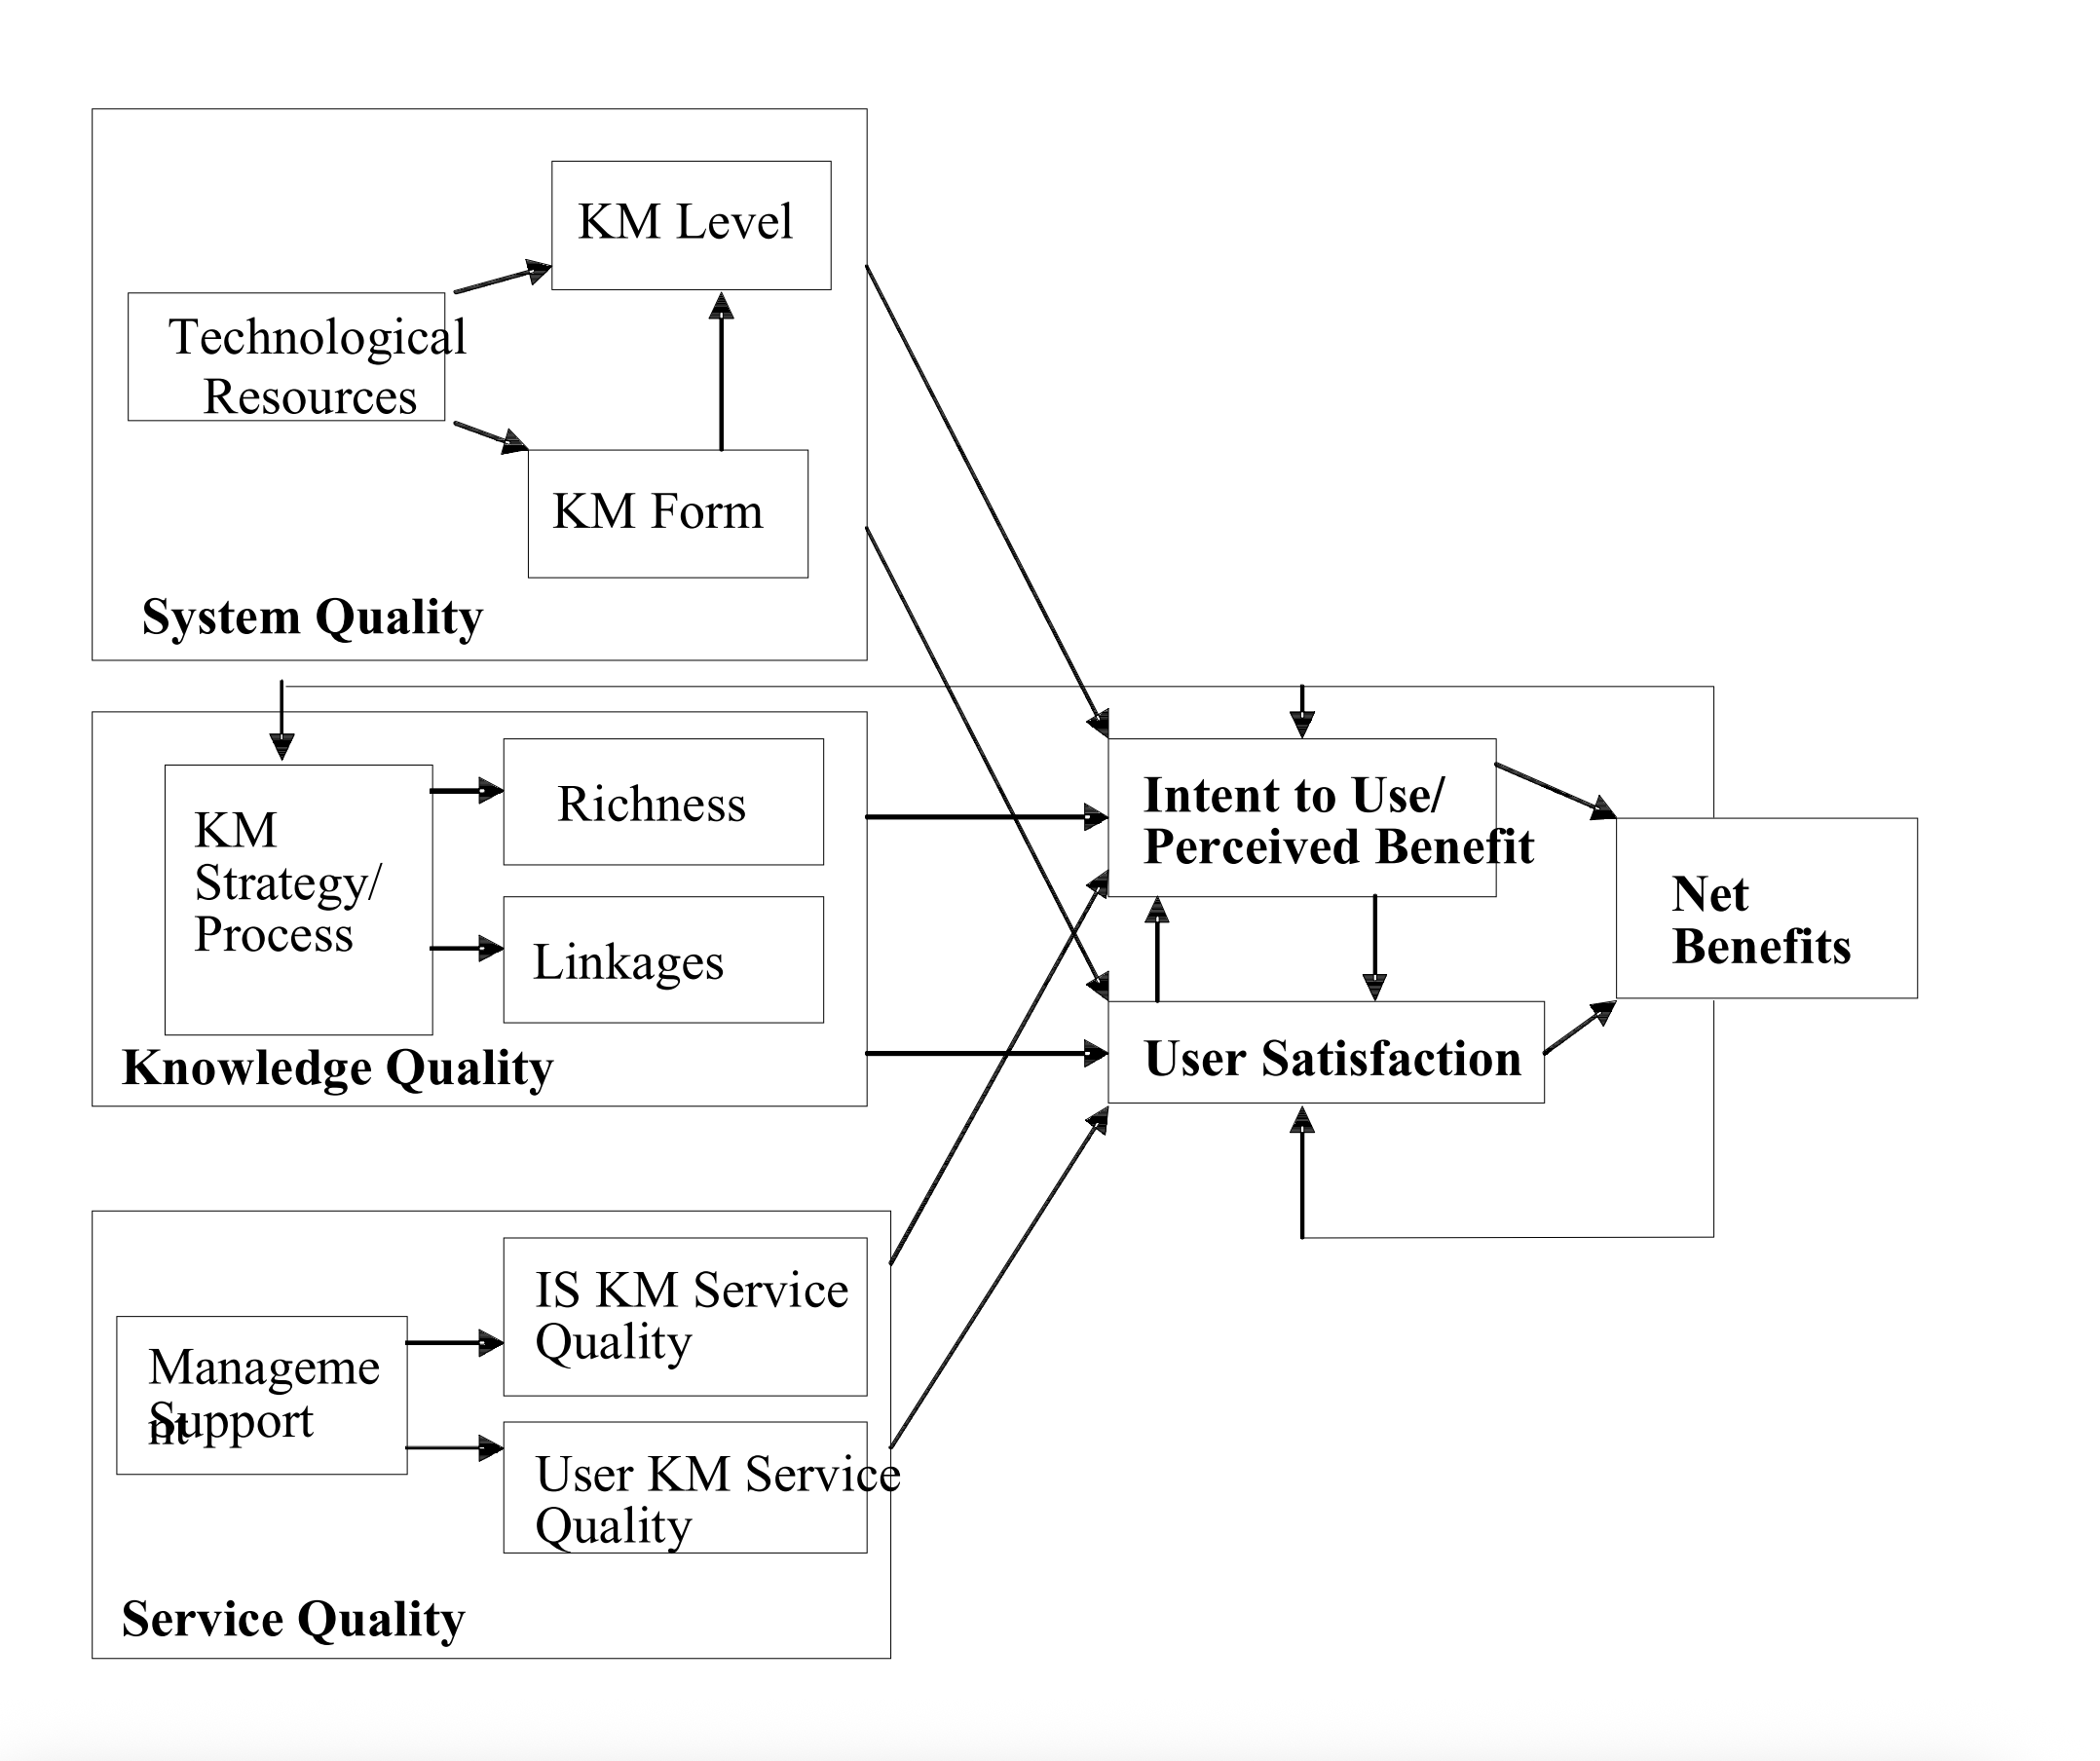
\includegraphics[width=1\linewidth]{knowledge_management_success.png}
    \caption{Knowledge management success model by Jennex & Olfman}
    \label{fig:enter-label}
\end{figure}
The \textit{System Quality} dimension extends to contain the \textit{technological resources}, \textit{KM form} and the \textit{KM level}. \textit{Technological resources} define the capability of an organization to develop, operate, and maintain KM. This includes all kinds of technical conditions like the amount of experience available to develop, operate and maintain the KM, the underlying network infrastructure or the databases to hold the data use in KM. The \textit{KM form} refers to the extent to which knowledge and knowledge management processes are computerized and integrated. This is important since computerized KM processes are more effective than analogue ones as they make knowledge accessible everywhere at any time through a simple to use interface. The \textit{KM level} in the end refers to the ability to influence current activities. \textit{Technological resources} and the \textit{KM form} are both enablers for the \textit{KM level} and serve as a technical foundation for the ability of the KMS to influence the decision-making process.\\\\
The \textit{Knowledge Quality· dimension} consists of three subsidiary factors too - the \textit{KM strategy/process}, the \textit{Richness} of the captured knowledge and the \textit{Linkages} among the knowledge components. The \textit{Knowledge strategy/process} factor is the basis for the two other factors and means looks at the organizational processes organizing the knowledge management and to which extend these processes are formalized. \textit{Richness} on the other hand evaluates the accuracy and timeliness of the knowledge itself - one could say it is the quality of the actual knowledge. Linkages refer to how accessible the knowledge is through things like knowledge and topic maps etc.\\\\
The \textit{service quality} dimension determines if users of the KMS are provided with sufficient support to use the KMS effectively. It consists of three parts aswell. The \textit{management support} refers to the provision of adequate resources for the KM the organization aswell as the creation of knowledge-sharing organization culture by the organization's management. User KM service quality refers to the support provided by the user organization in order to train the users to use the KMS effectively. On the other hand the IS KM service quality refers to the support provided by the  IS organization to allow users to use the KM aswell as maintaining it. This includes the building, setup and maintaining the KM infrastructure ensuring availability, reliability and security of the KMS provided.\\\\
All three dimensions - the \textit{system quality}, \textit{knowledge quality} and the \textit{service quality} influence similar to the original ISSS the \textit{Intention to use} as well as the \textit{User Satisfaction} and cause a \textit{net benefit} in the end. The KMS success model makes a small difference by replacing the actual usage with \textit{perceived benefit} to highlight the importance of the distinction between mandatory and voluntary use.
\section{Generative AI Systems in organizations}
Since we now know what determines the success of KMS in organizations like enterprises, we are going to have a closer look at the GenAI systems that are used to support KM in an organization, find out what they are used for and which factors define their quality.\\
AI in general is hard to define. For now we will follow the definition by Marvin Minsky and define Artificial Intelligence as "the science of making machines do things that would require intelligence if done by men" \parencite{MinskyBritannica}. In other words, AI systems are systems that show some form of intelligent behavior similar to human intelligence. Machine learning (ML) is a subfield of AI and describes the analysis of huge amounts of data \parencite{Lund2023}. Neural networks are models used in ML to perform this analysis. They imitate the human brain by using interconnected layers of artificial neurons (or nodes) to process information \parencite{Lund2023}. Generative AI (GenAI) is one kind of ML model approach that uses a neural network with a vast number of layers to generate new data based on training data \parencite{Lund2023}.
Large Language Models are one flavor of GenAI models. These models are trained on huge corpora of text and are capable of many text-processing tasks. The workflow using these LLMs is as follows: A user submits a request, known as a prompt, to the LLM, and the LLM generates a response based on its training data and the prompt \parencite{Lund2023}.\\
The GenAI system we will focus on throughout this thesis is a retrieval-augmented generation (RAG) system. These systems utilize external data sources like web pages, other organizational KMS, or third-party sources through retrieval algorithms \parencite{AWS_RAG}. The retrieved context is then passed alongside the user's query to a large language model (LLM) that generates an answer grounded on the retrieved knowledge. Such RAG systems can be used for open-domain question answering and can be used for knowledge work in an organization as they make (proprietary) knowledge available to an LLM \parencite{Lewis2020}.\\
\subsection{Advantages of RAG systems for organizational KM}
One problem of LLMs that do not use RAG is that they can only provide the data they were trained on. This causes them to become outdated. As we know from the KMS success model, an organization must be able to access up-to-date information using their KMS. RAG systems can provide this by utilizing up-to-date knowledge sources for their generation.\\
Another issue with LLMs is that they tend to hallucinate if they don't know the answer to a user's query or apply a pattern from the training data incorrectly. Since RAG systems bind the LLMs they use to the information provided by the retrieval algorithms, they reduce hallucinations, allowing a user to verify the answer provided by the LLM by double-checking the sources used by the RAG system. This way, the RAG approach improves the accuracy of LLMs.\\
Since RAG systems can query various data sources at once, they provide good linkages to other KMS as well. Following the KM- and IS success model, RAG systems seem like a pretty good choice when it comes to KM. \\
\subsection{Challenges for RAG systems in organizations}
However, realizing the full potential of RAG systems in an enterprise context requires significant effort. Enterprises typically have high requirements concerning not only the output quality but also compliance regulations, the integration of various data sources, and other factors. In the following analysis, we will examine some of the issues encountered in RAG systems used in enterprises and assign them to the quality dimensions of the ISSM. \\
A formal taxonomy of failure points for a RAG system, created based on three case studies, highlights seven distinct issue types related to \textit{Information quality} \parencite{Barnett_Kurniawan_Thudumu_Brannelly_Abdelrazek_2024}. These challenges range from fundamental data gaps, where the required information is simply missing from the knowledge base, to retrieval failures where required documents are not ranked highly enough by the retrieval algorithm or are lost during context consolidation. Further down the pipeline, the Large Language Model (LLM) might fail to extract the correct answer from the provided context. Finally, even if factually correct, the generated answer may have the wrong format, an incorrect level of specificity, or be incomplete, failing to fully satisfy the user's query \parencite{Barnett_Kurniawan_Thudumu_Brannelly_Abdelrazek_2024}.\\
Three other case studies demonstrate these theoretical \textit{Information quality} related issues in the real world too. In a 2023 case study, a RAG system implemented in a major healthcare organization began to produce a series of potentially harmful treatment suggestions that contradicted current medical standards. This occurred because its knowledge base contained outdated medical guidelines, inconsistent drug interaction databases, and incomplete patient history records \parencite{NStarX_Inc._2025}. This case highlighted the direct risks to patient safety. In another example, an investment firm's RAG system provided contradictory advice on securities regulations, potentially leading to compliance violations. An investigation found the knowledge base contained regulatory documents from multiple jurisdictions without proper geographic tagging, superseded regulations that had not been archived, and inconsistent interpretations of the same rule. The firm faced potential regulatory scrutiny and was forced to suspend the system, resulting in millions of dollars in lost productivity and increased manual oversight \parencite{NStarX_Inc._2025}. Similarly, a telecommunications chatbot began providing customers with incorrect billing information and outdated service plans. The root cause was traced to duplicate customer records, outdated product catalogs with discontinued services, and inconsistent pricing data across regional databases. \parencite{NStarX_Inc._2025}\\
Another study highlights five key challenges that RAG systems face, especially in compliance-regulated enterprise environments \parencite{Bruckhaus2024RAG}.\\
The first of these is maintaining accuracy, consistency, and explainability. Given that RAG outputs in sectors such as finance or healthcare can carry legal or financial weight, they require a higher level of trustworthiness and accuracy. Furthermore, the systems must be able to explain how retrieved documents influence the final generated content and provide confidence scores to help users assess the reliability of the output.\\
Secondly, data security, privacy, and compliance are critical. Enterprises must ensure their RAG systems comply with strict regulations, such as HIPAA or GDPR, which require robust data encryption, access controls, and detailed audit trails to prevent the unauthorized disclosure of sensitive information.\\
A third significant \textit{system quality}-related challenge is the \textbf{scalability and performance} of the RAG application. Enterprise knowledge bases are typically vast and complex, spanning numerous formats and systems. RAG architectures must be able to efficiently index, update, and search these massive data sources while maintaining high performance and low latency.\\
Fourth, integration and interoperability with existing IT infrastructure are essential. RAG systems must be designed to seamlessly integrate with an organization's content management platforms and databases, often requiring flexible APIs and custom connectors.\\
Lastly, customization and domain adaptation are crucial for achieving high accuracy. Each enterprise uses a unique data schema, taxonomy, and domain-specific language. RAG systems must be adaptable, allowing for the fine-tuning of language models and retrieval algorithms to understand this specialized context and improve the relevance and coherence of the generated results. Adopting the RAG system to handle domain-specific requirements requires a high \textit{service quality} since the teams supporting the system have to perform customizations.\\
The study concludes that RAG systems need to be purpose-built, as general-purpose RAG systems cannot adequately handle these challenges.\\
In conclusion, while RAG systems offer immense potential for enhancing an organization's knowledge management, considerable effort is required to realize this potential. Since the issues affect all three quality dimensions of the ISSM, an ideal evaluation framework should provide evaluation features that concern all three of them.
\section{Evaluation and analytics frameworks}
Several frameworks already exist for evaluating the \textit{information quality} of a RAG system. A prominent open-source example is the RAGAS evaluation framework, which in its original version uses an "LLM as a judge" approach to determine quality metrics \parencite{Es_James_Espinosa_Anke_Schockaert_2024}. Here, \textit{Answer Relevance} assesses if the answer fits the question, \textit{Faithfulness} evaluates if the retrieved documents support the answer, and \textit{Context Relevance} measures if the retrieved documents are relevant to the question. The framework has since been expanded to include a broader range of metrics, including some that are not model-based; however, a complete list is beyond the scope of this section. Other open-source solutions, such as ARES \parencite{Saad_Falcon_Khattab_Potts_Zaharia_2024}, also rely on LLM-based evaluation models.

Proprietary services also exist, such as Google's Gen AI Evaluation Service available on GCP, which uses a mix of LLM-based and computation-based metrics to assess RAG system quality \parencite{GoogleGenAIEvaluation}. This shows that using an LLM to evaluate RAG quality is a common and established practice, an approach that is also adopted in the evaluation dashboard developed in this thesis.

However, the frameworks mentioned above focus exclusively on RAG quality, which corresponds solely to the \textit{Information Quality} dimension of the IS Success Model. This thesis aims to cover the other quality dimensions as well. Existing systems often achieve a broader analysis through the integration of general analytic tools, e.g., Google Analytics \parencite{GoogleAnalytics}. Such tools enable the tracking of detailed user interactions, providing a more comprehensive picture of system usage. For instance, \textit{System Quality} can be assessed by measuring end-to-end page load times or tracking client-side errors to gauge performance and reliability. \textit{Service Quality} can be analyzed by tracking feature usage and monitoring engagement with advanced features to understand how users interact with a system.

The goal of this thesis, therefore, is to develop a dashboard that combines both approaches. It aims to move beyond a narrow focus on RAG-specific \textit{Information Quality} to provide a foundation for a holistic analysis of all quality dimensions of the ISSM.
% --  --  --  --  --  --  --  --  --  --  --  --  --  --  --  --  --  --  --  --  --  --  -- %
% --  --  --  --  --  --  --  --  --  --  Methodology  --  --  --  --  --  --  --  -- --%
% --  --  --  --  --  --  --  --  --  --  --  --  --  --  --  --  --  --  --  --  --  --  -- %
\chapter{Methodology}
The research methodology is based on the DSR approach, which involves the definition, development and evaluation of artifacts in iterative cycles. DSR aims to develop innovative solutions for specific problems and to test these solutions in real-world contexts \parencite{Peffers2007}.\\
\subsection{Problem Identification and Motivation}
In the first phase of the DSR approach, the need for support in evaluating the RAG system using a holistic approach following the ISSM was identified. It was determined that system administrators require insights that enable them to better assess the current performance and quality of the RAG application and draw conclusions about the measures that must be taken to improve it. Examples of such measures include employee training, enhancing the knowledge base, or improving the RAG mechanism itself.
\section{First iteration - Definition of valuable insights}
In the first iteration, specific software features were defined to support system administrators in managing the system. This was done in collaboration with the developers of the investigated RAG software during several joint workshops.
\subsection{Define Objectives of Artifacts}
In a first workshop, initial ideas for evaluating the RAG application were collected, and its current data situation was analyzed to determine what additional data must be gathered to implement the automated analysis. The developers were presented with the foundational principles of Information Systems Success (ISSS) and Knowledge Management Systems (KMS) success. They then developed ideas related to both topics in small groups and afterwards discussed their findings in a plenary session. Through this process, the objectives for the evaluation of the RAG system were clearly established
\subsection{Development of Artifacts}
Based on the developers' ideas, specific concepts for software features were developed and then classified into the quality categories of the IS Success Model (ISSM).
\subsection{Demonstration and Evaluation}
In a second workshop, the developed concepts were presented to the developers and feedback on them was gathered. Additionally, the individual software features were prioritized with the categories low, medium and high to ensure that the subsequent implementation phase could focus on developing and delivering the most important ones.
\section{Second iteration - Implementation of features}
In the second iteration, the developed software concepts were technically implemented and integrated into the existing RAG application.
\subsection{Define Objectives of Artifacts}
First, different technical implementation solutions were developed and presented to the development team once again. Feedback was gathered, and a decision was made on how the features should be technically implemented.
\subsection{Development of Artifacts}
Subsequently, the software features were implemented and integrated into the existing RAG application. Technical reviews took place to validate the correctness of the created software features.
\subsection{Demonstration and Evaluation}
Finally, the created software features were presented to the development team in a final workshop, and feedback was gathered.
% --  --  --  --  --  --  --  --  --  --  --  --  --  --  --  --  --  --  --  --  --  --  -- %
% --  --  --  --  --  --  --  --  --  --  Results  --  --  --  --  --  --  --  --  --  -- %
% --  --  --  --  --  --  --  --  --  --  --  --  --  --  --  --  --  --  --  --  --  --  -- %
\chapter{Results}
In the following chapter, we are going to elaborate on the concepts for software features created during the workshops and how they have been implemented in the RAG application. Feedback from the developer team and their prioritization of the features will be discussed as well.
\section{Description of the RAG system used in the study}
To provide a basis for further investigation, this section describes the features of the Retrieval-Augmented Generation (RAG) system under examination. The system is designed for enterprise use, making company-specific knowledge accessible to employees through a conversational interface powered by LLMs.

\subsection{System Architecture and Technology Stack}
The system is deployed on the Google Cloud Platform (GCP) \parencite{GoogleCloudDocumentation} and utilizes Vertex AI Search \parencite{GoogleVertexAISearch} for the initial document retrieval from its knowledge base. The relevance of the retrieved documents is subsequently optimized by the Vertex AI Reranker \parencite{GoogleReranker}. For the generation component, the system is capable of integrating various LLMs through the LangChain framework \parencite{LangChain}. Given its deployment on GCP, Google's Gemini models \parencite{GoogleGemini} are typically employed for response generation.

A central architectural feature of the system is the implementation of distinct \textbf{Use Cases} that are customized units capable of handling requests to a specified set of data. The customization allows the system to provide context-aware responses by augmenting the generation prompt with use-case-specific information, such as a specialized glossary or other supplementary data like a use-case-specific tonality. Each Use Case is associated with a specific selection of \textbf{Knowledge Assets}, which are custom compilations of \textbf{Knowledge Sources}. A Knowledge Source contains information on a particular topic and is technically linked to a Datastore in Vertex AI Search, which performs the underlying retrieval. The user requests are organized as follows: A user can start a thread within a use case. This thread can contain multiple chats that are linked to it. The user's requests are connected to a chat in turn. A use case and the data used in a use case is managed by a so called use case admin who is a trained employee of the company using the RAG system.

\subsection{Retrieval and Query Enhancement Features}
The system incorporates several advanced features to enhance the retrieval process:

\begin{itemize}
    \item \textbf{Query Splitting:} The user's search query is semantically decomposed into multiple sub-queries. A separate retrieval process is executed for each sub-query to ensure every semantic aspect of the user's query is covered \parencite{Chan2024}.
    
    \item \textbf{Query Reformulation:} The system supports the reformulation of user queries to add necessary context, e.g., from previous questions \parencite{Setty2024}.
    
    \item \textbf{Metadata Filtering:} The search performed by Vertex AI Search can be refined by applying a metadata filter. This allows for the retrieval to be constrained to only those documents that match specific attributes \parencite{Setty2024}.
\end{itemize}

\subsection{User Interface and Interaction Features}
The system provides a range of interactive features to enhance the user experience and workflow integration:

\begin{itemize}
    \item \textbf{Question Suggestions:} After an answer is generated, the system proposes alternative and potential follow-up questions to the users initial question that the user can select with a single click.
    
    \item \textbf{Document Viewer:} The documents retrieved during the search process can be viewed in an integrated file viewer and are available for download too.
    
    \item \textbf{Feedback:} Users can provide individual feedback on their satisfaction with the LLM responses.

    \item \textbf{Copy Function:} Users can copy the answer provided by the LLM using a Copy Button
    
    \item \textbf{Quick Actions:} The system offers "Quick Actions," which are clickable shortcuts that allow users to perform subsequent tasks with the generated information, such as creating an email or generating a summary.
\end{itemize}
\section{Software features}
This chapter presents the results of the developer workshops, namely the resulting concepts and their contribution to the GenAI success evaluation framework, as well as the prioritization and feedback by the developer team. Each concept is explained in terms of the quality dimensions that it can be used to measure. While many concepts allow Use Case administrators to improve the system across multiple quality dimensions, they are assigned to the dimension for which they are most suitable.
\subsection{Mostly system quality related concepts}
\subsubsection{Response Time Measurement}
The first concept for determining the system quality of the RAG application is the measurement of its response time, defined as the duration from the submission of a user's query to the delivery of the complete answer. For a comprehensive analysis, this measurement should incorporate not only the raw duration but also key system factors to assess their impact. These factors include the specific language model (LLM) being used and whether features such as Query Splitting or Query Reformulation were activated for the request. Using this feature, Use Case administrators can identify performance trends and retrospectively evaluate the impact of their own decisions on the response times of the RAG system. Furthermore, it enables them to assess better how various system factors affect the response time. These insights can, in turn, be used to train employees on the effective use of the system, for example, by providing better guidance on the performance implications of choosing a particular language model. By evaluating the response time of the system, Use Case administrators can draw conclusions on the performance of it and whether the \textit{technological resources} provided are suitable for the system, which is a key aspect of \textit{system quality}.

For the visualization of this data, a time-series diagram is proposed. The x-axis would represent the time and the y-axis the measured response time. To improve readability and highlight long-term developments, the chart should be smoothed, for instance, by displaying daily averages. The interface should also include interactive filters that allow for the inclusion of the different system factors. These filters would enable users to display data subsets, such as showing only the response times associated with a specific LLM or with Query Splitting enabled/disabled.

During the workshop, the development team assigned a \textbf{medium priority} to this feature. In their feedback, they noted that while the feature would be straightforward to implement, they suspected that overall response times would not vary significantly. Therefore, they hypothesized that this analysis would likely not yield major conclusions.

\subsubsection{Error Rate Monitoring}
A second concept proposed to evaluate system quality focuses on monitoring error rates to assess system stability and reliability. The core metrics to be captured are the absolute count and the percentage of user queries that result in a system error. For a more granular analysis, these error metrics can be combined with the system factors (LLM selection and the activation state of Query Splitting and Reformulation) and with the different predefined error types and messages of the system. By analyzing the error rates of the system, Use Case administrators can conclude the overall stability of the system, which is yet another critical \textit{system quality metric}. By providing the development and operations team of the RAG application with insights into frequent errors, this feature partly contributes to the \textit{IS KM service quality} of the RAG system, as well, since service processes carried out by the RAG system's vendor, such as bug fixes, are enhanced.

The visualization proposed for these data is again a time-series diagram. The x-axis would represent time, while the y-axis would display the amount or percentage of system errors. The interface is designed to be interactive, featuring filtering options for both system factors and error types. This allows for detailed analysis, such as comparing the error rates of different language models or analyzing the impact of query splitting and query reformulation on error rates.

The workshop feedback showed different views on this feature's usefulness and priority. One group assigned it a \textbf{high priority}. They argued that system errors are a major problem that can stop people from using the application and cause them to lose interest. This view highlights the feature's role in keeping users engaged. A second group assigned it a \textbf{medium priority}, seeing it mainly as a diagnostic tool for developers. For them, the main benefit was helping the development team find and fix technical issues faster. This group strongly recommended that this monitoring view should be for internal use by the development team only. They reasoned that showing raw error statistics to Use Case administrators or end-users could damage their trust in the system, which is not in the interest of the RAG systems vendors. In the end, the feature was assigned a \textbf{medium priority} since the arguments from the critical perspective predominated the other ones.
\subsection{Mostly information quality related concepts}
\subsubsection{Topic Map}
To better understand what information users are looking for, the concept of a "Topic Map" was developed. This feature is designed to visualize the main topics that appear in the RAG system. The map can display topics from three different data sources: the user queries themselves, the content of the documents retrieved by the system, or the knowledge assets that were accessed. By making the most important topics visible to the use case admins, the \textit{information quality} and following the KM success framework \textit{richness} and \textit{linkages} can be enhanced, e.g., by optimizing the underlying data for these topics. \textit{User KM service quality} can be improved as well, since the Use Case administrator can analyze whether users are choosing a suitable use case for their requests and provide guidance if needed.

In the idea discussed in the workshop, the map is displayed as a bubble plot, where each bubble represents a specific topic. The positioning is semantic, meaning that topics with similar meanings are positioned closer to each other, and related topics are grouped by color. The size of each bubble shows how frequent or prominent a topic is. The feature also includes a time filter, which allows administrators to see how user interests and queried topics change over a specific period.

The development team rated the overall Topic Map feature as a \textbf{high priority}, but they assigned different levels of importance to analyzing each of the three data sources:

\begin{itemize}
    \item \textbf{Topics from user queries:} This received a \textbf{high priority}. The team agreed that this view would provide the most valuable insights into what knowledge users are actively searching for, which lets use-case-administrators identify their interests and potential knowledge gaps in the system.
    
    \item \textbf{Topics from retrieved documents:} This was given a \textbf{medium priority}. The feedback noted that because documents can be very large and cover many subjects, the detected topics might not be very precise, making this analysis less useful.
    
    \item \textbf{Topics from knowledge assets:} This was rated as a \textbf{low priority}. The team reasoned that use-case-administrators already know what their knowledge assets are about, so a visualization of these topics would likely offer little new insight.
\end{itemize}
\subsubsection{Task Type Analysis}
To analyze user intent and behavior, the concept of a "Task Type Map" was introduced. In contrast to the Topic Map, which focuses on \textit{what} users ask, this feature classifies queries based on \textit{how} users interact with the system. The primary goal is to understand the different ways the application is used, which can provide valuable insights for improving user workflows.

The initial concept proposed displaying this data in a bubble plot, similar to the Topic Map, where bubble size would represent the frequency of each task type. However, the team questioned this visualization during the workshop. They pointed out that the semantic relations of the different task types do not matter in this case since only predefined task types will be assigned to the user queries which makes a semantic interpretation of the different task types themselves obsolete. As a more practical alternative, the team suggested that a \textbf{bar chart} would be better suited to compare the frequencies of these distinct task categories.

However, making the most frequently used task types visible to the Use Case administrators can improve the \textit{information quality} by optimizing the RAG system and its underlying data to better fulfill these task types. It also enhances the \textit{service quality}. Use Case administrators can interpret how their users use the RAG system by analyzing the most relevant task types. This enables them to support their users better.

Despite the discussion on the best visualization method, the development team assigned the Task Type Map a \textbf{high priority}. They agreed that understanding the primary ways the system is used is crucial. This information can help to improve and streamline common user workflows and better tailor the system to user behaviors.
\subsubsection{Quality of Retrieval and Response}
An important concept for evaluating the system is the measurement of its output quality. This feature focuses on assessing both the relevance of the retrieved documents and the quality of the generated response. The main goal is to establish metrics for how well the system performs to ensure that users receive accurate and helpful answers. By analyzing the quality evaluations, Use Case administrators can draw conclusions about how well the system performs in terms of information \textit{richness} and \textit{information quality}, identify trends, and also conclude how their own past decisions influenced the \textit{information quality}. This way, they can enhance it over time.

The discussion highlighted that there is no single and perfect way to measure quality automatically. Therefore, the team proposed different approaches that could suite the quality measurement:

\begin{itemize}
    \item \textbf{AI as a Judge:} Using a separate LLM or another AI model to automatically score the quality of a given response.
    \item \textbf{Binary Metrics:} Implementing simple, automated checks. For retrieval, this could mean checking if any retrieved text has a certain similarity score to the query. For the response, it could be a check to see if an actual answer to the question was provided or if the LLM responded with no answer.
    \item \textbf{User Behavior Analysis:} Using indirect metrics, such as counting the number of follow-up or rephrased questions. A high number could suggest that the initial response was unsatisfactory.
\end{itemize}

The results would be displayed in a time-series chart with the x-axis representing the time and the y-axis representing the quality of the system's responses. The system factors (the model selection, Query Splitting and Reformulation) also be included as filtering options as described before to see how they affect quality.

The development team unanimously assigned this feature a \textbf{high priority}, describing it as one of the most critical factors for the RAG success. The team emphasized that guaranteeing high-quality responses is essential for user retention - if users do not get good answers, they will stop using the system.
\subsubsection{Combined Quality and Topic/Task Analysis}
Another concept proposed in the workshop was a combination of the previous ideas on quality measurements and topic/task type analysis into a single visualization. This "Combined Quality and Topic/Task Analysis" was designed to connect the system's performance quality directly with the specific topics or task types being handled. The goal is to identify patterns and understand if the \textit{richness} and \textit{information quality} vary for different topics in user queries. By directly connecting output quality to topics, Use Case administrators can pinpoint \textit{information quality} issues and improve the underlying data for the topic if needed.

This feature uses the bubble plot from the "Topic Map" feature as its foundation. In the idea discussed in the workshop the positioning of the bubbles (semantic similarity) and their color (topic clusters) remains the same, as does the sliding time window for dynamic analysis. The crucial change lies in the meaning of the bubble size. Instead of representing the frequency of a topic, the size of each bubble now represents the average retrieval or response quality for that topic. For example, a large bubble could signify a topic with consistently high-quality answers, while a smaller bubble might indicate a topic where the system often performs poorly.

The development team assigned this combined view a \textbf{high priority}. The key benefit they identified was the ability to find patterns between query types and the quality of the results. By using this map, administrators could quickly see if a specific topic area suffers from low-quality answers or if certain task types are handled better than others. This information is critical for making targeted improvements and focusing development efforts on the areas where the system is weakest.
\subsubsection{Combined Task Type and Topic Analysis}
Another concept was proposed to analyze the relationship between the topics users ask about and the tasks they are trying to perform. This feature is designed to identify the specific user intents that are associated with different topics. This provides a deeper understanding of user behavior within different knowledge domains which allows Use Case administrators to improve the \textit{richness} and \textit{information quality} by optimizing the RAG-system and its underlying documents as well as the \textit{User KM service quality} by allowing them to understand better how users use the system.

For this analysis, a new visualization method was suggested: a \textbf{heatmap}. In this chart, the rows would represent the various topics identified in the system, while the columns would represent the different task types (e.g., knowledge query, summarization). The color intensity of the cell where a topic and task type intersect would indicate how frequently that specific combination has occurred. For example, a darker cell would show that a particular task is performed very often in connection with a given topic.

The team agreed that this analysis could provide "good insights" into user behavior and assigned a \textbf{medium to high priority}. Understanding which tasks are most common for high-interest topics could help administrators better structure content or create more relevant "Quick Actions" to improve the user experience for those specific topics.
\subsection{Mostly service quality related concepts}
\subsubsection{User Interactivity Tracking}
To evaluate the service quality of the application, a concept for tracking user interactivity was discussed. The idea is to monitor and count a wide range of specific user events that happen during a session. This approach tries to make the whole user interaction interpretable and therefore includes analyses interactions like copying an answer, viewing a source document, or providing direct feedback. This enables Use Case admins to understand how their users use the system and by this improves their ability to support their users, which means that the \textit{User KM service quality} is improved. Furthermore, since the use of the RAG system is voluntary, we can associate the \textit{actual use} of the system and its functionalities with the \textit{intention to use}, which is a strong indicator for \textbf{net benefits} and IS success overall.

The data would be visualized in a time-series diagram, showing the frequency of these different events over a selected period. A key aspect of this concept is to also provide the use case admins with context or an interpretation of what each measurements for the different interaction types could mean. For example, a high number of users opening source documents might indicate they are actively verifying the system's answers, while frequent follow-up questions could suggest that the initial answers lacked sufficient detail.

The team assigned this feature an overall \textbf{medium priority}, which led to a detailed discussion about which specific events were the most valuable to track. A central point of the debate was data redundancy. Some team members argued for a lower priority on tracking metrics like the number of questions or raw feedback counts, as this data was already present in other specialized dashboards.

However, other members rated certain interactive events as \textbf{high priority} because of the unique insights they offer. The events considered most important were:
\begin{itemize}
    \item \textbf{Opened Source Documents:} This was rated high because it clearly shows if users find the retrieved sources relevant enough to investigate further.
    \item \textbf{Provided Feedback (Positive/Negative):} This was also seen as high priority because it is the most direct way to capture user sentiment and serves as a "good measurement" of perceived quality.
    \item \textbf{Deep-Dive Follow-up Questions:} This was considered a useful indicator of answer quality, as a high frequency might signal that the initial responses were incomplete.
\end{itemize}
Ultimately, the consensus was to focus on tracking the most insightful events that were not already available elsewhere.

A specific challenge that arose from tracking user interactivity was how to correctly interpret follow-up questions. The team needed a way to distinguish between "deep dive" questions, which indicate positive user engagement, and questions asked because the system's previous response was unclear or unhelpful. Two main approaches were considered: using a simple heuristic (e.g., assuming system-suggested "Follow-Up questions" are deep dives, while user-rephrased "alternative questions" are not) or employing an AI model as a "judge" to classify the question's intent based on context.

The recommendation from the workshop was to adopt a pragmatic hybrid strategy. The consensus was to start with the "simple distinction" method first, as it is easy to implement and has no operational cost. If this heuristic proves insufficient for reliably separating the two question types, the team could then explore using an AI judge as a second step. This approach was favored due to concerns that the AI judge would be expensive to run and might not guarantee reliable results.
\subsubsection{Knowledge Gap Detection}
The last concept proposed for measuring service quality is "Knowledge Gap Detection," which aims to identify areas where the system or the users may lack adequate knowledge. The goal is to highlight two distinct types of knowledge gaps:

\begin{enumerate}
    \item \textbf{Knowledge gap within the system:} This occurs when the topic of a user's question aligns with the topic of a relevant knowledge asset, but the system fails at retrieving relevant documents. This suggests an internal deficiency in the system's ability to retrieve the correct information, despite the knowledge theoretically existing within its accessible sources. This could be due to issues with indexing, retrieval algorithms, or the structuring of the knowledge assets themselves. In this case Use Case admins can improve the \textit{richness} and \textit{information quality} of the RAG system by improving the RAG pipeline itself or the underlying data.
    \item \textbf{User knowledge gap:} This refers to situations where the topic of the user's question does not align with the topic of any relevant knowledge asset. This indicates that the user is searching for information that is either not present in the system's knowledge base or is not categorized in a way that allows for effective retrieval. This gap highlights potential areas where user training on the system scope might be beneficial. In this case, Use Case admins can improve the \textit{User KM service quality} of the RAG system by assisting their users in choosing a suitable use case for their requests.
\end{enumerate}

For visualization, it is proposed to track the occurrences of these knowledge gap types over time and display them in a time-series diagram. The x-axis would represent time, while the y-axis would indicate the frequency of each gap type. This allows administrators to observe trends in knowledge gaps and identify if certain periods or topics are more prone to these issues.

During the workshops, the development team assigned a \textbf{medium to high priority} to the "Knowledge gap detection" feature, specifically emphasizing its importance for analyzing system data. The ability to identify internal system knowledge gaps was considered crucial for pinpointing areas where the RAG mechanism or the underlying knowledge base need improvement. The mechanism for checking topic alignment -- whether topics "fit together" -- was discussed. The proposal uses semantic similarity measures (e.g., cosine similarity of embeddings) to compare the topics extracted from user queries, retrieved documents, and knowledge assets. If the similarity score falls below a predefined threshold, a mismatch, and thus a potential gap, is flagged.
\subsection{Implementation Roadmap}
Finally, after discussion with the development team, the following roadmap for implementing the proposed software features was agreed upon:
\begin{enumerate}
    \item Implementation of the tracking system for the user interactions
    \item Implementation of a caching logic for performance optimization
    \item Topic maps
    \item Quality of retrieval/responses
    \item Combination of quality and topic/task type maps
    \item Task type maps
    \item Knowledge gap detection
    \item Combination of task types and topics
    \item Interactivity analysis
    \item Response time analysis
    \item Error rate analysis
\end{enumerate}
This roadmap was particularly important because it was clear from the beginning that not all of the proposed features could be implemented within the timeframe of this thesis due to time constraints. Therefore, prioritizing the concepts was essential to ensure that the most important features could be developed and integrated first.
\section{Description of the implemented software features}
The following section describes how the software features were implemented in the RAG system. For each feature, the description will cover its integration into the user flow as well as its technical implementation.
\subsection{Tracking system and GDPR compliance}
The first thing we need to evaluate the user interactions is a tracking system to record them. The foundation of the tracking system developed during the thesis is BigQuery \parencite{GoogleBigQuery}, a scalable, high-performance data warehouse solution from Google. As it is natively integrated into the Google Cloud Platform (GCP), it is well-suited for analyzing the application's user data.

To record the data, a Google Cloud Run service \parencite{GoogleCloudRunService} is used, which receives data from the RAG application's Vue-based frontend via HTTP and writes it to BigQuery. These HTTP calls are executed asynchronously and in parallel with the rest of the application's requests. This ensures that the tracking process does not interfere with the performance or usability of the RAG application.
The foundation of the tracking system is Google's BigQuery, a scalable, high-performance data warehouse solution. As it is natively integrated into the Google Cloud Platform (GCP), it is well-suited for the analysis of user data.\\
\\
The tracking system supports the recording of the following interaction types:
\begin{itemize}
    \item \textbf{Question Asked:} A user submits a new query.
    \item \textbf{Documents Received:} The system retrieves a set of source documents.
    \item \textbf{Answer Received:} The LLM generates a final response.
    \item \textbf{Quick Action Used:} A user uses Quick Action.
    \item \textbf{Alternative Question Asked:} A user asks an alternative question.
    \item \textbf{Follow-Up Question Asked:} A user selects a system-suggested follow-up question.
    \item \textbf{Source Document Opened:} A user opens a source document to view its contents.
    \item \textbf{Feedback Provided:} A user gives feedback on a generated answer.
    \item \textbf{Model Selected:} A user changes the language model for the conversation.
    \item \textbf{Query Reformulation Used:} The query reformulation feature is activated.
    \item \textbf{Query Splitting Used:} The query splitting feature is activated.
    \item \textbf{Copy Button Clicked:} A user copies the text of the generated answer.
    \item \textbf{Filtering Used:} A user applies a metadata filter for the search.
\end{itemize}
To maintain the context of a conversation, interactions belonging to a chat or thread within a Use Case are also tracked. In BigQuery, the chat is recorded as a "SessionChat" and the thread is recorded as a "Session". This structure makes it possible to determine which interactions were triggered within the same chat or thread.

For compliance with GDPR (DSGVO) \parencite{DSGVO_2024} regulations, these chats and threads are pseudonymized. This means that pseudonymized IDs are used to prevent a chat or thread from being linked back to a specific user, removing the possibility of subsequent re-identification. Furthermore, a table was created containing a justification for why the recording is necessary for every single data point that is tracked to make the tracking system GDPR compliant.
\subsection{Data flow and data preprocessing}
\begin{figure}
    \centering
    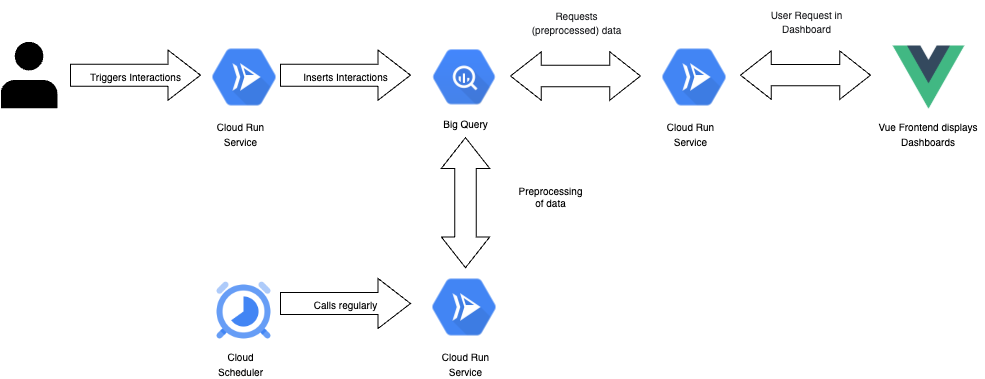
\includegraphics[width=1\linewidth]{images/DataFlow_Bachelorthesis.drawio.png}
    \caption{Dataflow}
    \label{fig:enter-label}
\end{figure}
The data flow for the dashboard system, as illustrated in the preceding diagram, can be broken down into three primary processes:

\begin{enumerate}
    \item \textbf{Data Collection:} As described before, when a user interacts with the system these interactions, such as asking a question or clicking a button, triggers an event that is sent via an HTTP request to a \textbf{Cloud Run Service}. The purpose of this service is to receive these events and insert the raw interaction data into \textbf{BigQuery}.

    \item \textbf{Data Preprocessing:} To ensure the dashboards are performant and can display analytics quickly, the data is preprocessed since some of the calculation steps have a long runtime. Instead, an automated preprocessing job is run. A \textbf{Cloud Scheduler} is configured to trigger a \textbf{Cloud Run Service} at configurable regular intervals. This service reads the raw data from \textbf{BigQuery}, performs the necessary calculations to prepare the data for displaying in the dashboard, and writes the processed data back into new tables within \textbf{BigQuery}.

    \item \textbf{Data Visualization:} When a user opens a dashboard in the \textbf{Vue Frontend}, a request is sent to a \textbf{Cloud Run Service} that functions as a backend for the dashboard. This service queries the prepared, preprocessed data from \textbf{BigQuery}. It then sends this data back to the \textbf{Vue Frontend}, which renders the final charts for the user using the Apache eCharts library. This architecture ensures that user requests are served quickly, as the complex data processing has already been handled before.
\end{enumerate}
\subsection{The Welcome Page}
For all the following features, screenshots are available in the appendix.
The first page a Use Case administrator sees when accessing the dashboard is the Welcome Page. This page serves as a central starting point, providing instructions on how to use the dashboard system and offering short descriptions for each of the available analytical metrics. As shown in the screenshot, the user receives guidance on the general workflow in a "Getting Started" section. Above this, a selection of cards introduces the different metrics of the dashboard. From here, the administrator can begin their analysis by selecting one of the metrics to explore.
\subsection{Answer Quality}
\subsubsection{User Flow}
The answer quality feature was implemented to provide Use Case administrators with a time-series chart, as outlined in the initial feature concept. This chart allows them to observe trends in answer quality over time and draw conclusions about the success of their own measures. The diagram displays the four quality metrics: Relevance, Completeness, Accuracy, and Faithfulness. A description for each metric can be found in the prompt template provided in the appendix. Furthermore, an end-user study needs to be conducted to validate the choice of these metrics, as they are generally used to assess RAG quality. To give a clearer overview, the values are smoothed to show the daily averages over the selected period. In addition to filtering by Use Case and date range, the dashboard also displays the overall average values for each metric above the chart, enabling a quick analysis of the entire period. The chart is interactive, allowing users to hide individual lines for better focus and use tooltips to analyze specific data points in detail.

\subsubsection{Technical Implementation}
During the workshops, three technical options were proposed for this feature: evaluation using binary metrics, analysis of user behavior, or using an AI model as a "judge". The binary metric and user behavior analysis were considered to be less accurate proxies for quality, as both methods only indirectly evaluate the content of the generated response. This is obvious in the case of user behavior analysis, which only looks at the user's subsequent questions, not the answer itself. In this way, a detailed explanation of the answer quality is not possible. The binary analysis is also limited, as it primarily checks if the RAG system could assemble relevant information, but does not assess the qualitative aspects of that information.

Therefore, the decision was made to implement the AI evaluation variant. In this implementation, a language model is provided with the user's query, the retrieved source documents, and the final answer during the preprocessing step of the data flow. Using a prompt template that contains detailed instructions for determining the different quality metrics, the AI "judge" then assesses the answer and calculates the scores. The prompt template can be found in the appendix. The calculated scores can then be accessed from the frontend via an HTTP request to the Cloud Run backend that accesses the results stored in BigQuery.
\subsection{Document quality}
\subsubsection{User Flow}
The Document Quality feature was implemented in a manner similar to the Answer Quality feature, based on the concepts developed in the workshops. For each user query, this dashboard displays a time series that shows several metrics related to the retrieved documents: the average, highest, and lowest relevance scores, as well as the total number of documents. The technical basis for relevance is described in the next section. These values are presented as smoothed daily averages in a time-series chart to make it easier for the Use Case administrator to analyze trends. The dashboard also includes options to filter by Use Case and time period, and the overall averages for each metric are displayed as KPI cards above the chart. The chart itself is interactive, allowing administrators to use tooltips for detailed analysis of specific data points and to toggle the visibility of individual time series.

\subsubsection{Technical Implementation}
To determine the document quality metrics, the implementation uses the relevance scores that are calculated by the system's reranker during the retrieval process. This approach was chosen to avoid the additional costs associated with using another AI model for a separate evaluation. These reranker scores, which are generated by a cross-encoder, already provide an assessment of how well the retrieved documents match the user's query. From these scores, the system calculates the average, highest, and lowest relevance values for each query, as well as the total number of documents retrieved in the preprocessing step. It can then request these aggregated values.
\subsection{Topic maps}
\subsubsection{User Flow}
The Topic Maps are presented to the user as a bubble plot. In contrast to the proposal from the workshop in the implemented visualization, each bubble represents an individual user question -- not a whole topic -- allowing for a more detailed overview. The position of each bubble in the chart is determined by its semantic meaning, with topically similar questions appearing closer together than dissimilar ones. Furthermore, the questions are thematically grouped using a clustering algorithm. Each cluster of questions is assigned a unique color on the chart and is displayed with a descriptive title in the legend. The dashboard allows administrators to filter the view by Use Case and date range, enabling them to analyze how the thematic composition of user queries changes over time. Tooltips are also available to show details for each individual question bubble.

\subsubsection{Technical Implementation}
The Topic Maps are generated during preprocessing by first embedding all user queries using the \texttt{gemini-embedding-001} model in its clustering mode \parencite{GoogleEmbedding001}. These embeddings are then clustered using the HDBSCAN algorithm. To achieve robust results across varying amounts of data, the input parameters for HDBSCAN, specifically \texttt{min\_cluster\_size} and \texttt{min\_samples}, are dynamically adjusted based on the total number of queries being analyzed. This adaptive approach ensures sensible clustering for both small and large datasets. The HDBSCAN algorithm is a good choice for this use case as it automatically determines the number of topics (clusters) and effectively isolates irrelevant queries as noise. This eliminates the need to pre-specify the number of clusters, a key limitation of methods like K-means, making it ideal for discovering topics in an exploratory way \parencite{Baligodugula2025}. To overcome the issue that HDBSCAN is not well-suited for high-dimensional data, UMAP is applied before the HDBSCAN algorithm to reduce the dimensions beforehand.

After clustering, a language model uses a prompt template to generate a descriptive title for each cluster based on a sample of its questions; this title is then displayed in the legend. Finally, to visualize the 3072-dimensional vectors produced by the embedding model, their dimensionality is reduced to two dimensions using the UMAP again, allowing them to be plotted on the 2D chart. The UMAP algorithm is known to handle high-dimensional vectors well, which makes it a good choice in the case of high-dimensional embedding vectors compared to, for example PCA or t-SNE \parencite{McInnes2020}.
The resulting clusters, cluster names and 2-dimensional coordinates stored in BigQuery can be requested by the frontend using the Cloud Run backend.
\subsection{Task type analysis}
\subsubsection{User flow}
The task type analysis was implemented as a time-series diagram. It was noted in the workshop that a bubble plot would not fit to this feature, because the semantic relationship between the discrete task types is not important. A bar chart was suggested as an alternative. However, a time-series chart was ultimately implemented because, in addition to showing numerical values, it also allows for the analysis of trends over time. This chart displays the days on the x-axis and, on the y-axis, the number of times an individual task type occurred in user queries on a given day.

The system recognizes and displays the following task types:
\begin{itemize}
    \item Question Answering
    \item Summarization
    \item Content Creation
    \item Code Generation
    \item Rewriting
    \item Translation
    \item Data Analysis
    \item Other
\end{itemize}
\textbf{Note:} These task types are a collection of types that are recognized as typical task types for GenAI applications and could potentially appear in requests to the examined RAG system. Yet, they should be evaluated in an end-user study.\\
\\
The dashboard also provides options to filter by Use Case and time period. The chart is interactive, supporting tooltips for detailed analysis and the ability to toggle the visibility of each time series. Furthermore, to provide the at-a-glance summary that a bar chart would have offered, the overall percentage distribution of each task type for the entire selected period is displayed above the chart.

\subsubsection{Technical implementation}
Technically, a language model assigns each user query to a specific task type during preprocessing. This is done using a prompt template that contains detailed instructions and descriptions for each category. The prompt template receives the user's question, the final answer, and the retrieved documents as input parameters. To save costs, the quality evaluation (as described previously) and the task type assignment were combined into a single prompt. Therefore, for this classification task, the language model receives more inputs than just the user query. In the end the assigned task types can be requested by the frontend using the Cloud Run backend that accesses the results stored in BigQuery.
\subsection{Combining answer and document quality with topic maps}
\subsubsection{User Flow}
In the Topic Map view, administrators can display collected document and answer quality scores directly on the bubble plot. Since each user question is represented as a single bubble, and varying bubble sizes would be difficult to distinguish across all questions, bubble size as proposed in the workshop isn't used as a quality indicator. Instead, when a quality metric is chosen from a dropdown menu, the bubbles change color. Greener colors indicate better quality (closer to 1), while redder colors signify poorer quality (closer to 0), replacing cluster membership as the color's meaning. Additionally, tooltips update to show the relevant quality metrics for each question instead of cluster information.

Additionally, a detail view is available which presents a table with an overview of either the document or answer quality metrics for all questions within a specific cluster. The administrator can select both the cluster and the set of metrics to be displayed using dropdown menus.

This feature allows for the identification of specific knowledge gaps for certain topics within a Use Case. By analyzing quality in the context of topics, a Use Case administrator can determine which subjects are being answered well and which are not. If a topic is performing unexpectedly poorly, the administrator can use this analysis to recognize the issue and initiate countermeasures, such as adding new source documents to the knowledge base.

\subsubsection{Technical Implementation}
Technically, this feature is enabled through simple \texttt{JOIN} operations in the BigQuery queries. This allows the quality metrics for each question to be queried and merged with the topic map data at the time of the request. Preprocessing is not needed.
\subsection{Combining quality with task types}
\subsubsection{User Flow}
The combination of quality and task types is also presented to Use Case admins as a time-series diagram. In this view, the administrator can select a specific quality metric (from either document or answer quality) using dropdown menus. The chart then displays the performance of this chosen metric over time, with each line representing a different task type (e.g., "Question Answering," "Summarization"). This allows for a direct comparison of how quality differs across various user intents.

As in the other dashboards, the data is smoothed by displaying daily averages. Users can filter the data by Use Case and time period. Above the chart, KPI cards display the overall average values for the relevant quality metrics across the entire selected period. The chart itself is interactive, offering tooltips for a detailed daily breakdown of quality per task type, and the ability to show or hide the lines for specific task types to focus the analysis.

\subsubsection{Technical Implementation}
Technically, the data for this view is queried using simple \texttt{JOIN} operations on the necessary tables in BigQuery during the user's request.
\subsection{Combination of task type and topics}
\subsubsection{User Flow}
The last implemented feature is the combination of task type and topic. This analysis is presented to the user as a heatmap. In this visualization, the horizontal axis represents the individual task types, while the vertical axis represents the respective semantic clusters. Each question that belongs to a specific task type and a specific cluster is counted in the cell where the two overlap. Cells with higher total values are colored more darkly than cells with lower values. It is also possible to filter the display for a specific time period and to restrict the view to a single Use Case.

\subsubsection{Technical Implementation}
Here as well, the data is queried through simple \texttt{JOIN} operations on the necessary tables in BigQuery during the user's request.

\subsection{Relative Operational Cost Comparison}
To assess the financial impact of the implemented analytics features, a detailed, relative comparison of operational costs per request was conducted. The analysis focused specifically on the additional Large Language Model (LLM) and embedding costs incurred by the new analytics pipeline for each user query. This additional cost was then compared to the baseline LLM cost of the main RAG query-response chain. To create a focused comparison, several cost factors were intentionally excluded, most notably data retrieval costs from the Datastore that cannot be traced back to a single request, as well as negligible costs from BigQuery and Cloud Run. This means the resulting percentages represent a \textbf{maximum relative increase}, since including the relatively high datastore costs would lower the final figure.

Two primary scenarios were analyzed to understand the cost impact under different conditions:

\begin{itemize}
    \item \textbf{Scenario 1: Simple RAG Chain.} The baseline was a simple query using one call to the most suitable Gemini model for Question Answering (\texttt{Gemini-2.5-Pro}). The additional analytics features require one call to a lower-cost model (\texttt{Gemini-2.0-Flash}) for quality and task type evaluation, and one call to the embedding model (\texttt{Gemini-Embedding-001}) for topic map analysis. In this scenario, the relative cost increase was calculated to be \textbf{24\%} \parencite{GoogleGeminiPricing}.

    \item \textbf{Scenario 2: Complex RAG Chain.} This scenario assumed a more advanced baseline chain that already included features like Query Reformulation and Splitting, which require several additional calls to smaller, faster models. When the same analytics features were added to this more expensive baseline, their relative cost increase was lower, calculated at approximately \textbf{18\%} \parencite{GoogleGeminiPricing}.
\end{itemize}
Detailed calculations can be found in the appendix.

From these scenarios, it was concluded that the analytics features add approximately \textbf{20\%} to the direct LLM-related costs, depending on the complexity of the underlying RAG chain. It is important to contextualize this increase: the cost is comparable to that of other advanced features already in the system. Furthermore, the analysis identified that the primary cost drivers for the entire system were Networking and Cloud Run services, not LLM usage. Therefore, the introduction of the new analytics features is not expected to significantly impact the total operational budget.

\section{Final Feedback from the Development Team}
Finally, the development team was asked to provide feedback on the implemented software features in a dedicated workshop. During this session, the fundamental goal of the thesis, evaluating GenAI Success, was recapped first. Following this, each new analytics feature was presented in a live demonstration, with an explanation of how it contributes to the overall evaluation goal. To conclude the workshop, the developers provided structured feedback by filling out a detailed questionnaire, the complete results of which can be found in the appendix.

Overall, the feedback from the development team was highly positive and constructive. The general design, interactivity, and visual presentation of the dashboards were praised, with comments describing them as well-designed and intuitive for technical users. The analysis of the detailed feedback revealed several key themes and areas for potential improvement:

\paragraph{Clarity and User Onboarding} A primary theme that emerged was the need for enhanced clarity, particularly for non-technical administrators. Recurring suggestions included adding more detailed legends to explain what metrics like "Faithfulness" mean and providing specific examples to help users interpret the scores. It was also noted that explaining the interdependencies between metrics -- for instance, how "Accuracy" and "Completeness" might influence "Faithfulness" -- could provide a deeper understanding, perhaps visualized as a funnel. Furthermore, the idea of adding automated, LLM-generated summary statements to explain the main takeaways from a chart in plain language was proposed to facilitate the access.
\paragraph{Actionability} A strong desire was expressed to connect high-level insights not just to deeper analysis, but to specific, operational actions. While the team suggested adding drill-down capabilities to trace an aggregated metric to its source, their feedback went further. There was a clear call to bridge the gap between identifying a problem and implementing a solution. Specific proposals included creating functionality to generate a new "Quick Action" directly from an identified, frequent user task, as well as the ability to overlay key events, such as software releases or pipeline updates, onto the quality trend charts. This would enable a direct correlation between development efforts and their impact on performance.
\paragraph{Visualization Optimization} While the charts were considered visually appealing, the team provided feedback on optimizing the choice of visualization for the specific data. Specific suggestions included making clusters in the topic map more visually distinct by drawing lines around them, using different shapes in line charts for better accessibility, and implementing more advanced user interface controls, such as an interactive "sliding window" to select date ranges directly within a graph.
\paragraph{Trust and Explainability in AI-Generated Metrics} The developers also provided a differentiated perspective on AI-based evaluations. They noted that an LLM evaluating its output is inherently prone to error and recommended adding disclaimers to manage user expectations. However, their main concern went beyond simple accuracy to the need for explainability. There was a desire not just to see a score, but to understand the reasoning behind it -- why the model considered a particular answer to be of low quality. This feedback highlights a need for systems that provide not just metrics, but also insight into the AI's decision-making process.\\
\\
In conclusion, from the development team's perspective, the implemented features provide significant value for assessing GenAI success and represent a strong foundation for future work. The feedback suggests that the primary focus for subsequent iterations should be on improving the onboarding experience for non-technical users and, most important, enhancing the actionability of the dashboards -- not only by enabling more granular drill-downs, but by creating direct pathways from analytical insights to operational improvements.

% --  --  --  --  --  --  --  --  --  --  --  --  --  --  --  --  --  --  --  --  --  --  -- %
% --  --  --  --  --  --  --  --  --  --  Discussion  --  --  --  --  --  --  --  --  -- %
% --  --  --  --  --  --  --  --  --  --  --  --  --  --  --  --  --  --  --  --  --  --  -- %
\chapter{Discussion}
The primary goal of this work was to develop an artifact in the form of a dashboard that automatically evaluates the success of an enterprise GenAI application and presents its findings to the use case administrators in a clear and meaningful way so that they can draw conclusions for the optimization of the RAG system. The discussion will begin by interpreting the key findings in the context of the initial research question. Afterwards, the limitations of the developed artifact and the research methodology will be critically examined. Finally, the implications for both theory and practice will be outlined, followed by an outlook on future research opportunities.

\section{Interpretation of the Results}
The central result of this thesis is the successful development and implementation of an analytics dashboard integrated into an existing enterprise RAG system. This artifact was designed to provide Use Case administrators with the necessary tools to evaluate and improve the success of their GenAI applications, directly addressing the initial research question.

\paragraph{Connecting to the IS Success Model} The implemented features can be directly mapped to the dimensions of the DeLone and McLean IS Success Model, which served as the theoretical foundation for this work.
\begin{itemize}
    \item \textbf{Information Quality} is addressed through the \textit{Answer Quality}, \textit{Document Quality}, \textit{Topic Map} and \textit{Task Type analysis} features. These dashboards provide direct insights into the relevance, accuracy, and completeness of the information provided by the system and allow administrators to identify knowledge gaps by analyzing the topics users are asking about. This directly operationalizes the "Richness" and "Linkages" components of the extended KMS success model by Jennex and Olfman.
    \item \textbf{System Quality}, while not the primary focus of the implementation due to prioritization, was conceptualized through features like \textit{Response Time} and \textit{Error Rate} monitoring. The implemented features, however, do contribute indirectly by providing data that can be used to diagnose system-level issues that affect information quality.
    \item \textbf{Service Quality} is reflected in the analysis of \textit{Task Types}, \textit{Topic maps} and the combined views. Furthermore concepts like the \textit{error rate monitoring}, \textit{knowledge gap monitoring} and \textit{interactivity analysis} have been conceptualized. By understanding how users interact with the system (e.g., which tasks they perform for which topics), administrators can better tailor the service, for example, by creating more relevant Quick Actions or improving user training.
\end{itemize}
Using the evaluation features of these three categories Use Case administrators can draw conclusions on their user's \textit{intention to use} and \textit{actual use}  as well as their \textit{satisfaction} with the RAG system and ultimately evaluate the \textit{net benefits} of it. By this, the implemented dashboard provides a solid foundation for the evaluation of IS success in a RAG context.\\
\\
The final workshop feedback confirmed that the development team saw a clear link between the implemented features and the goal of evaluating IS success. The features were perceived as providing a solid foundation for a comprehensive "Knowledge Analytics Engine."

\paragraph{Functionality and Value Added} The implemented artifact successfully translates abstract quality dimensions into specific, measurable metrics. The most valuable feature is the Topic Map combined with quality metrics. It moves beyond simple quality or performance checks and allows administrators to ask, "For which specific topic is our system failing?" This is a highly actionable insight that can directly lead to improvements, such as adding specific documents to the knowledge base. In contrast, features like the standalone quality dashboards provide scores that are harder to interpret without context. They signal that a problem exists, but they do not immediately point to the cause. Tracing these aggregated metrics to their sources by adding drill-down functionalities will improve the actionability of these features.

\section{Critical Reflection and Limitations}
The limitations of this thesis can be categorized into methodological and technical aspects.

\paragraph{Methodological Limitations}
\begin{itemize}
    \item \textbf{Evaluation Scope:} The evaluation of the artifact was conducted exclusively with the internal development team. While their feedback is valuable for assessing technical feasibility and the conceptual alignment with developer goals, it does not represent the perspective of the end-users -- the Use Case administrators. An end-user study in a real-world scenario should be the next step to validate and improve the dashboard's practical usefulness and apply DSR best practices. However, this was not possible during the thesis due to time constraints.
    \item \textbf{Partial Implementation}: Also, due to the time constraints of the thesis, not all concepts from the initial workshops could be implemented. Features like \textit{Response Time Analysis}, \textit{Error Rate Monitoring}, and \textit{Knowledge Gap Detection} were conceptualized but not realized. This means the implemented artifact provides a view that is heavily focused on Information Quality, while System Quality and Service Quality are less comprehensively covered.
\end{itemize}

\paragraph{Technical and Conceptual Limitations}
\begin{itemize}
    \item \textbf{Reliability of AI-based Evaluation:} The core of the answer quality evaluation relies on an LLM acting as a "judge." As pointed out by the development team, this approach has inherent limitations. An LLM evaluating another LLM's output can be unreliable and may not align with human judgment. Therefore, a disclaimer should be added to manage users' expectations.
    \item \textbf{Complexity vs. Intuitiveness:} The final feedback highlighted an important tension. The dashboards are powerful but also complex. A non-technical user will need to invest time to understand the metrics and how to interpret them. This suggests that the "Perceived Ease of Use" (PEU) might be a barrier, even if the "Perceived Usefulness" (PU) is high. The need for good help features and user onboarding is a direct consequence of this observation.
\end{itemize}

\section{Implications for Practice and Theory}
Despite the limitations, this thesis offers significant implications for both practical application and academic research in the field of Information Systems.

\paragraph{Practical Implications} The primary contribution for practice is a ready-to-use analytics tool that empowers organizations to make data-driven decisions about their enterprise GenAI systems. Use Case administrators can now:
\begin{enumerate}
    \item \textbf{Identify and address knowledge gaps within a use case} by seeing which topics are frequently requested but receive low-quality answers.
    \item \textbf{Optimize user workflows} by understanding the most common task types used and how they are used (e.g., for which topics). They can adapt use-case-specific information like the glossary to their users' needs.
    \item \textbf{Analyze the impact of their decisions} by using time series diagrams to identify influential events and match them against the changes they made.
    \item \textbf{Guide users to better outcomes} by analyzing their behavior. Suppose a user asks about a topic in a use case that does not support the topic. In that case, the administrator can identify that using the topic map and recommend a more suitable one to ensure they receive a high-quality answer.
\end{enumerate}
The cost analysis further showed that the financial impact of such an analytics suite is manageable, adding approximately 20\% to the LLM-related costs, which is a justifiable expense for the insights gained.

\paragraph{Theoretical Implications} This work contributes to the academic discourse by demonstrating an operationalization of the IS Success Model in the new context of enterprise RAG systems. It shows how the abstract dimensions of the model can be translated into specific, measurable metrics (e.g., "Faithfulness" as a metric for Information Quality). By employing the Design science research methodology, a well-structured framework has been used to create new artifacts reliably. Furthermore, this work adopts a new perspective on evaluating RAG applications shaped by the IS Success Model, which has not been used in prior research. Rather than focusing only on RAG quality, a more holistic perspective is taken -- based on the three quality dimensions of the ISSM -- which in turn guides the development of a dashboard that allows use case administrators to perform comprehensive analyses.

\section{Outlook and Future Research}
This thesis provides a solid foundation and opens up several paths for future research and development.

\textbf{Long-Term User Study:} The most important next step is to conduct a long-term study with Use Case administrators using the dashboards in a real-world scenario. This would enable an evaluation of the artifact's real-world impact on IS success and provide valuable feedback for further refinement.\\
\\
\textbf{Refining AI-based Evaluation:} Future research could focus on improving the reliability of the automated quality evaluation. This could involve developing more sophisticated evaluation pipelines, for instance, by incorporating a "self-reflection" step where the AI judge must justify its score, or by fine-tuning smaller, specialized models for the evaluation task to reduce costs and improve consistency.\\
\\
\textbf{Actionability:} A key suggestion from the feedback was to enhance actionability. Future work could focus on "closing the loop" by adding more drill-down capabilities to the dashboard, allowing users to trace issues to their sources. For example, a detailed view could be added to the quality charts that allows users to identify problems with the RAG quality.\\
\\
\textbf{Expanding the Scope:} Finally, the unimplemented features from the roadmap, such as \textit{Error Rate Monitoring} and \textit{Knowledge Gap Detection}, are next steps for expanding the dashboard's functionality to provide an even more holistic view of GenAI success.\\
\\
In conclusion, the developed artifact represents a significant step towards the systematic and automated evaluation of enterprise GenAI applications. The journey from raw data to actionable insight is complex, but this work has laid a solid and promising foundation for future exploration and improvement.

% --  --  --  --  --  --  --  --  --  --  --  --  --  --  --  --  --  --  --  --  --  --  -- %
% --  --  --  --  --  --  --  --  -- - Conclusion  --  --  --  --  --  --  --  --  -- --%
% --  --  --  --  --  --  --  --  --  --  --  --  --  --  --  --  --  --  --  --  --  --  -- %
\chapter{Conclusion}
The objective of this thesis was to design and implement a system for automatically measuring the success of an enterprise-level Retrieval-Augmented Generation (RAG) application from a new and more holistic perspective on RAG success, utilizing the ISSM. The project began with a series of collaborative workshops with the development team of the investigated RAG application to conceptualize a suite of analytics features tailored to the specific needs of the RAG system. Following this, a significant portion of these features was technically implemented, resulting in an integrated analytics dashboard within the application's admin panel. The technical solution was built on the Google Cloud Platform, leveraging BigQuery for scalable data warehousing, Cloud Run for efficient data processing, and a Vue-based frontend for interactive data visualization.

The implemented system provides insights into the three quality dimensions of the ISSM - \textit{system quality}, \textit{information quality} and \textit{service quality}. Key implemented features include dashboards for \textit{Answer Quality} and \textit{Document Quality}, which use AI-based evaluation to provide metrics like relevance and faithfulness. Furthermore, dashboards for \textit{Topic Map} and \textit{Task Type} analysis were developed to offer a deeper understanding of user interests and intents. These individual views were then combined into more powerful analytics tools that combine quality with specific topics and task types, allowing administrators to pinpoint knowledge gaps and areas for improvement. A cost analysis revealed that these new features incur a manageable, maximum overhead of approximately \textbf{20\%} on LLM-related costs.

The implemented analytics dashboard was presented to the development team for evaluation. The feedback was very positive, with the team confirming the high value and potential of the features for monitoring and improving the RAG system. The design, interactivity, and visual appeal of the dashboards were particularly praised.

The constructive feedback also highlighted several key areas for future enhancement. The most prominent theme was the need to improve clarity and user guidance for non-technical administrators through refined in-app explanations and user onboarding. A second major theme was the desire for greater actionability, primarily through the implementation of drill-down features that would allow users to trace an aggregated metric back to the specific documents or conversations that influenced it.

Due to the time constraints of this thesis, not all conceptualized features were implemented. The established roadmap provides a clear path for future development. Future work should prioritize:
\begin{itemize}
    \item Enhancing user guidance, for example by implementing the suggested LLM-generated "insight statements" for each chart.
    \item Developing drill-down capabilities to make the data more actionable.
    \item Carry out an end-user study with the use case admins to test the dashboard in real-world scenarios
\end{itemize}

In conclusion, this work delivered a solid foundation for GenAI success measurement based on the ISSM. The implemented system provides the business with valuable insights into its RAG application, and the detailed feedback from the development team creates a clear and validated path for future iterations to further increase its value.
% --  --  --  --  --  --  --  --  --  --  --  --  --  --  --  --  --  --  --  --  --  --  -- %
% --  --  --  --  --  --  --  --  --  --  Appendix  --  --  --  --  --  --  --  --  -- --%
% --  --  --  --  --  --  --  --  --  --  --  --  --  --  --  --  --  --  --  --  --  --  -- %
\chapter*{Appendix}
\addcontentsline{toc}{chapter}{Appendix}        %Kapitel bekommt keine Nummerierung und wird trotzdem
                                                                %ins Inhaltsverzeichnis aufgenommen
% Fortsetzung der römischen Seitennummerierung
\pagenumbering{Roman}
\setcounter{page}{\value{seitenzahlroemisch}}
\section{Statement on the use of AI for the creation of this thesis}
This paper was written independently and its language was revised with the assistance of Gemini and Grammarly. Cursor was used as a coding assistant during the artifact development.

\printbibliography


%\affidavit


\end{document}
